\newpage
\section{Selection}%TODO 图片转笔记, 课上摸了
\subsection{Lower Bound for Finding Median}

Trival lower bound: $n-1$

but there are crucial comparison and non-crucial comparison.

Adversary: give non-crucial comparison

\begin{figure}[H]
    \centering
    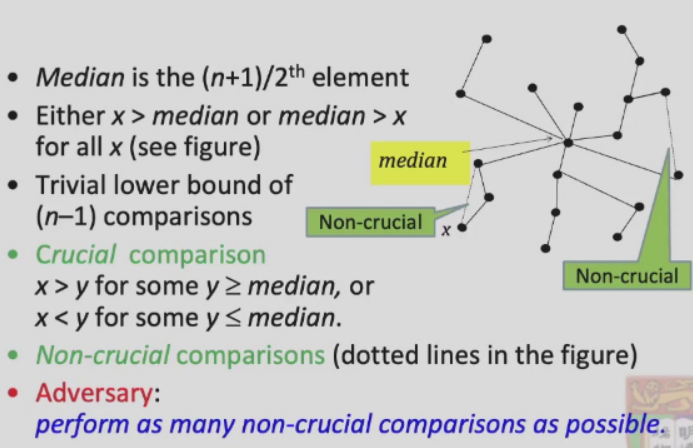
\includegraphics[width=0.309\textwidth]{pic/DAA3/Finding Median}
    \caption{Finding Median}
\end{figure}

\subsubsection{Adversary}
\begin{figure}[H]
    \centering
    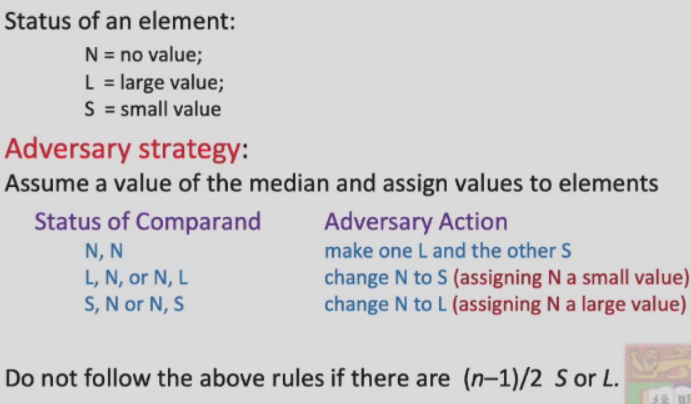
\includegraphics[width=0.309\textwidth]{pic/DAA3/Adversary}
    \caption{Adversary}
\end{figure}

lower bound = crucial + non-crucial = $3(n-1)/2$

\begin{example}
    Median of 5 elements
    \begin{itemize}
        \item sorting: 7
        \item lower bound: 6
    \end{itemize}
\end{example}

\subsubsection{Median Algorithm}
$O(n\log n)$
\begin{figure}[H]
    \centering
    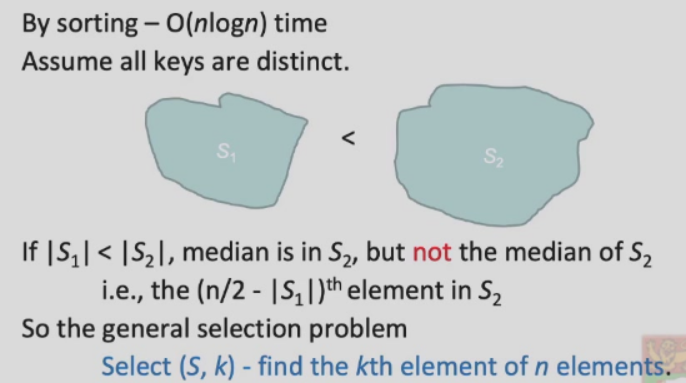
\includegraphics[width=0.309\textwidth]{pic/DAA3/Median Algorithm}
    \caption{Median Algorithm}
\end{figure}


Divide $S$ into ...

\begin{figure}[H]
    \centering
    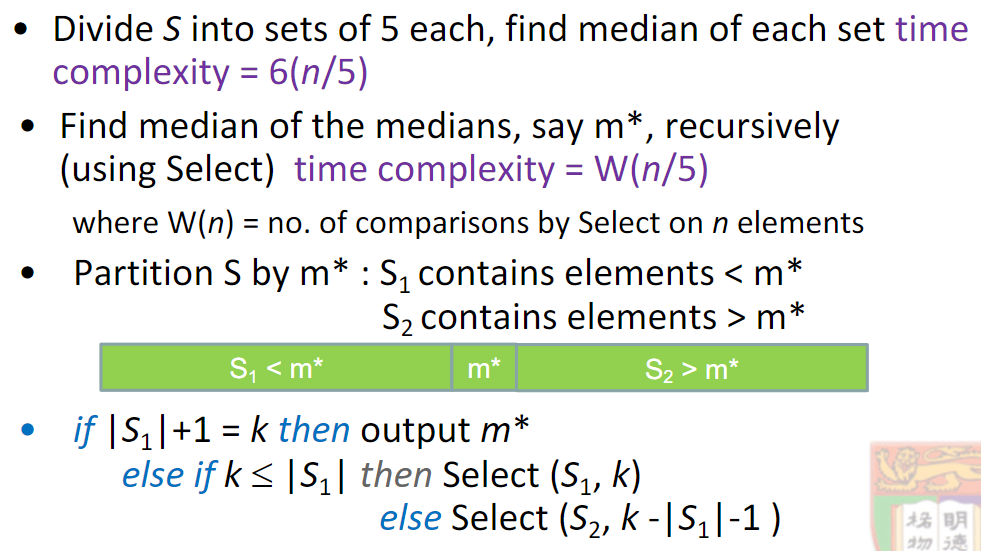
\includegraphics[width=0.309\textwidth]{pic/DAA3/Select(S,k)}
    \caption{Select(S,k)}
\end{figure}

%TODO group of 5 fig

\subsubsection{Time Analysis}
归纳法证明, 线性算法

\begin{figure}[H]
    \centering
    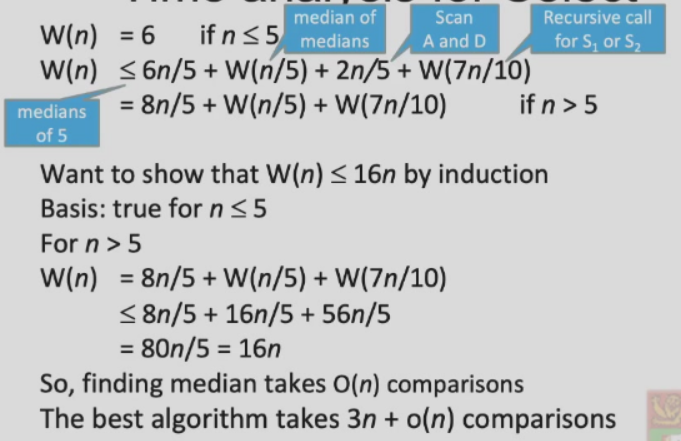
\includegraphics[width=0.309\textwidth]{pic/DAA3/Time Analysis}
    \caption{Time Analysis}
\end{figure}

\subsection{Finding the \texorpdfstring{$k$}.th Largest/Smallest Elements}
$k$-selection problem

sorting : $O(n\log n)$

use Max heap
% 这里有一个线性建 heap, 是复杂度算出来的线性
\begin{figure}[H]
    \centering
    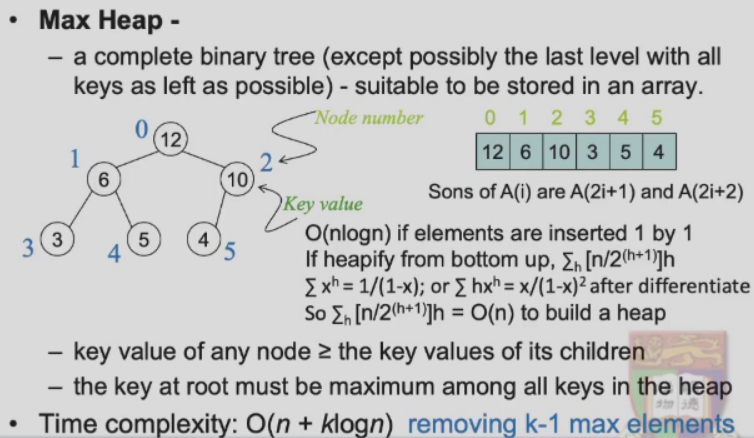
\includegraphics[width=0.309\textwidth]{pic/DAA3/Max heap}
    \caption{Max heap}
\end{figure}

And we can also find max use mim heap

\begin{figure}[H]
    \centering
    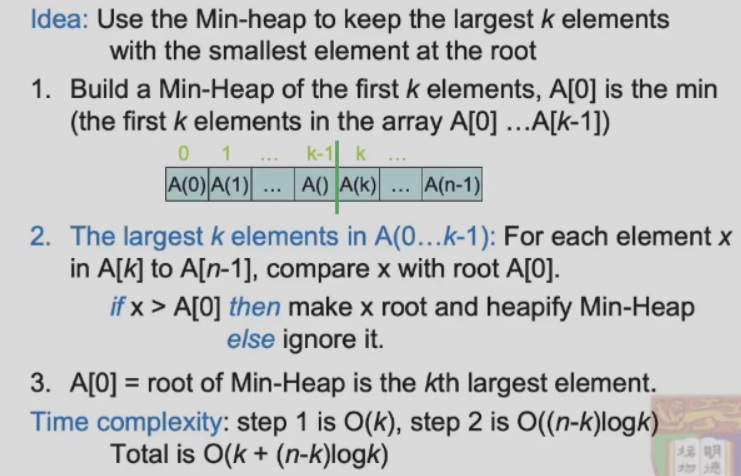
\includegraphics[width=0.309\textwidth]{pic/DAA3/mim heap}
    \caption{mim heap}
\end{figure}


\subsubsection{Lower Bound(Sketch)}

\begin{figure}[H]
    \centering
    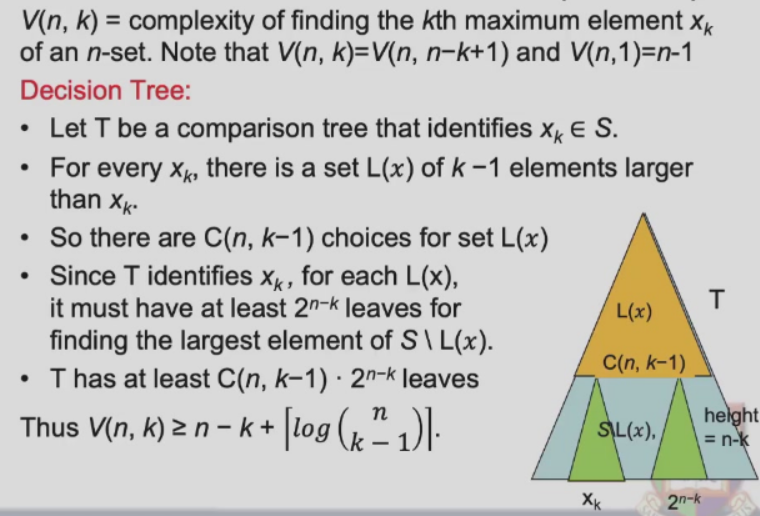
\includegraphics[width=0.309\textwidth]{pic/DAA3/Lower Bound}
    \caption{Lower Bound}
\end{figure}
 
\begin{figure}[H]
    \centering
    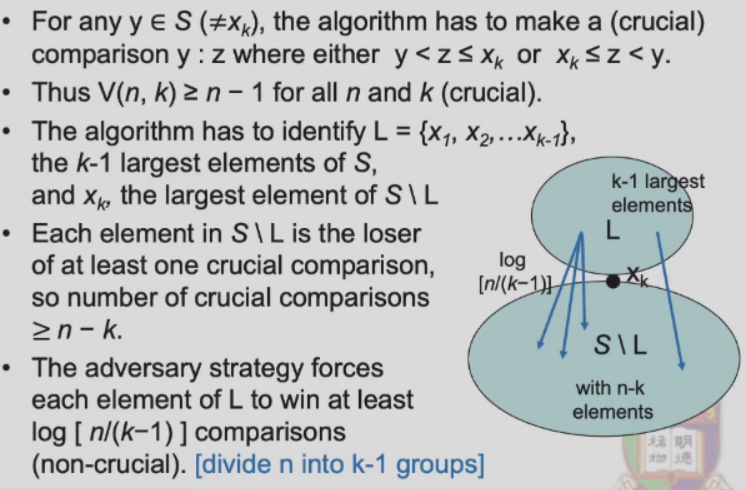
\includegraphics[width=0.309\textwidth]{pic/DAA3/Adversary selection}
    \caption{Adversary selection}
\end{figure}

\begin{theorem}
    \begin{align*}
        V(n,k)\ge n-k +(k-1)\left\lceil \log\frac{n}{k-1} \right\rceil
    \end{align*}
\end{theorem}

\begin{figure}[H]
    \centering
    \begin{subfigure}{0.48\textwidth}
        \centering
        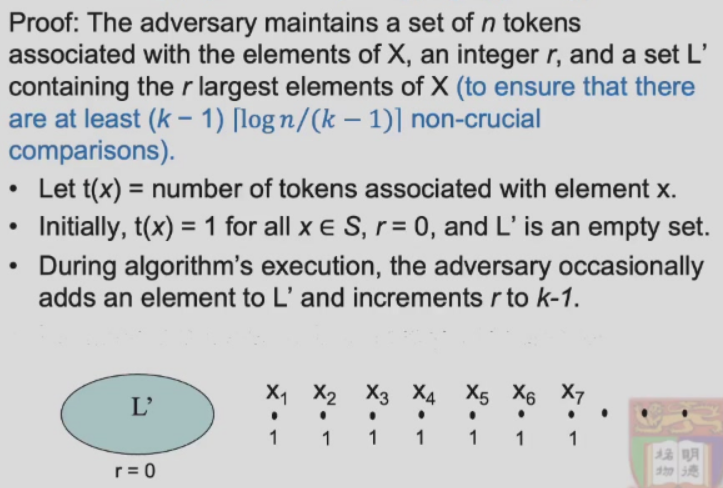
\includegraphics[width=0.618\textwidth]{pic/DAA3/theoremproof1}
    \end{subfigure}
    \begin{subfigure}{0.48\textwidth}
        \centering
        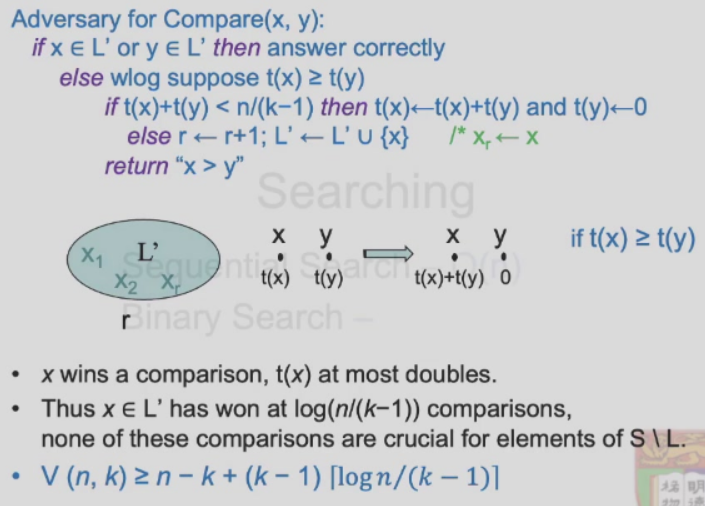
\includegraphics[width=0.618\textwidth]{pic/DAA3/theoremproof2}
    \end{subfigure}
    \caption{theorem proof}
\end{figure}
